\documentclass[11pt,letterpaper]{article}
\usepackage[utf8]{inputenc}
\usepackage{hyperref}



%----- Configuración del estilo del documento------%
\usepackage{epsfig,graphicx}
%% Ruta de las imágenes
\graphicspath{{resources/}}
\usepackage{geometry}
\usepackage{fancyhdr}
\usepackage{lastpage}
\pagestyle{fancy}
\usepackage{float}
\fancyhf{}

% Encabezado
\fancyhead[L]{\textit{Práctica 4: Cifrados Clásicos}}

% Pie de página
\fancyfoot[L]{\textit{Facultad de Ciencias, 2025-I}}
\fancyfoot[R]{\textit{Criptografía y Seguridad}}

%-------------------------------------------------%


%%Para la bibliografía
\usepackage[style=apa, backend=biber]{biblatex}
\addbibresource{referencias.bib}



\begin{document}

\newgeometry{left=2cm,right=2cm,top=1.8cm,bottom=2.3cm} % Cambiar los márgenes solo para la primera página

\begin{titlepage}
    \begin{center}
        \rule{17cm}{0.1mm}
    \end{center}
    \begin{center}
        \begin{minipage}{3cm}
            \begin{center}
                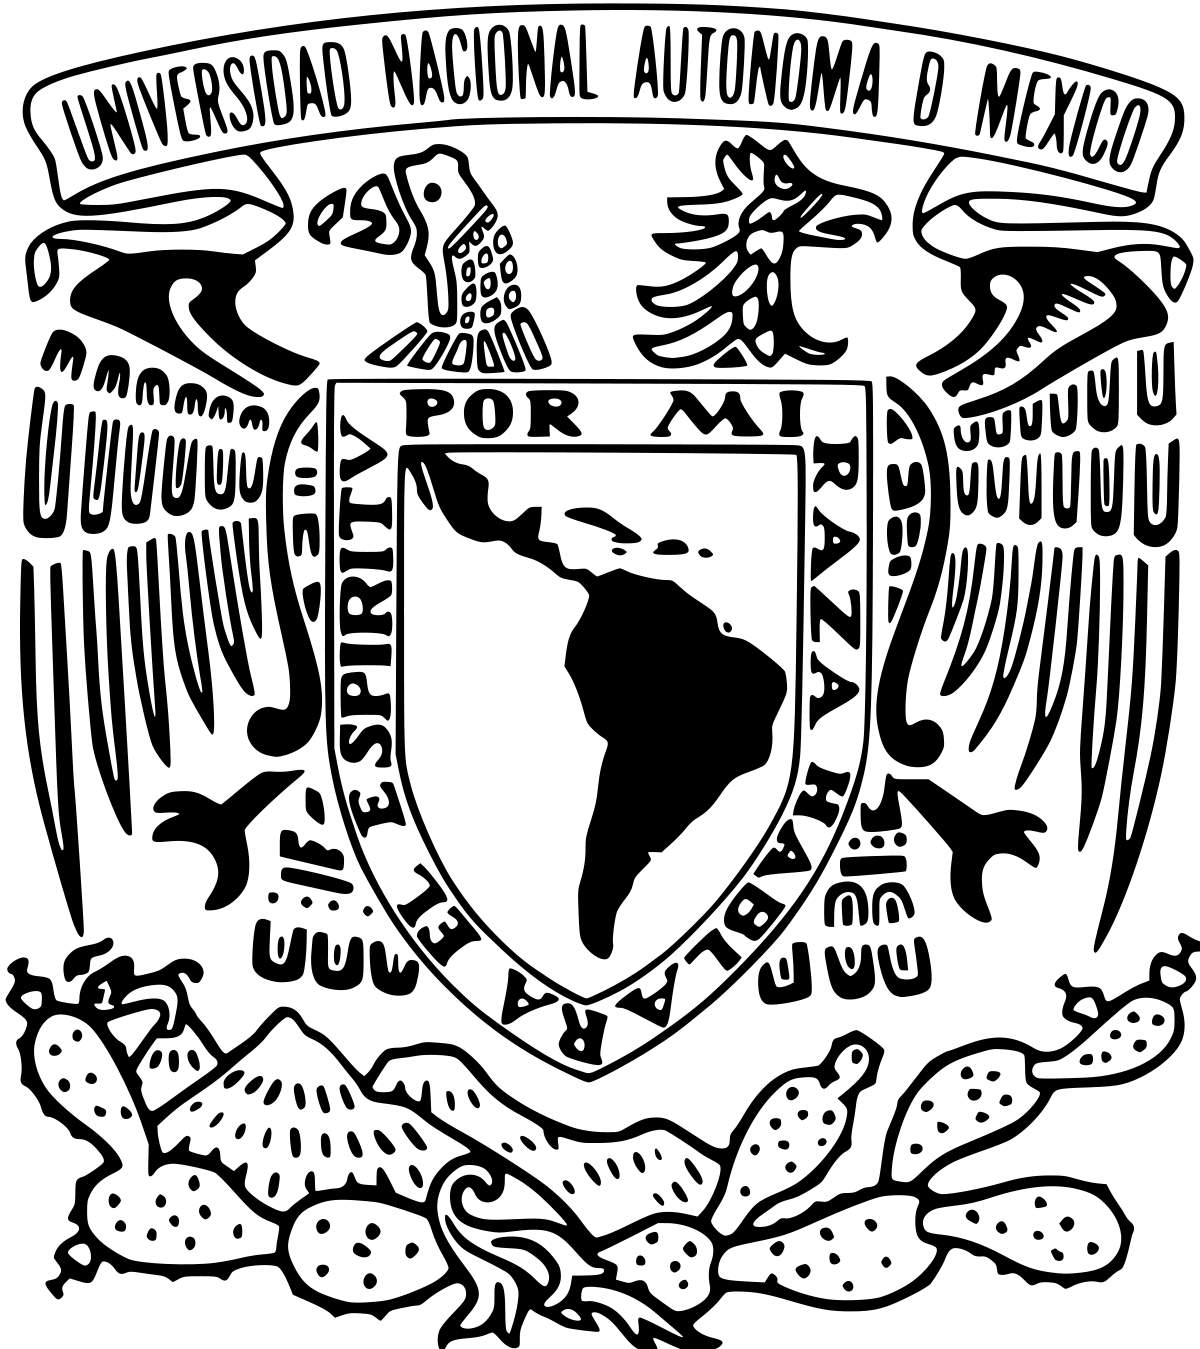
\includegraphics[height=3.4cm]{Logo_UNAM.png}
            \end{center}
        \end{minipage}\hfill
        \begin{minipage}{10cm}
    
            \begin{center}
                \large
                \textbf{ Universidad Nacional Autónoma de México}\\[0.1cm]
                \textbf{Facultad de Ciencias}\\[0.1cm]
                \textbf{Criptografía y Seguridad}\\[0.1cm]
                \textbf{Semestre 2025-1}\\[0.1cm]
            \end{center}
        \end{minipage}\hfill
        \begin{minipage}{3cm}
            \begin{center}
                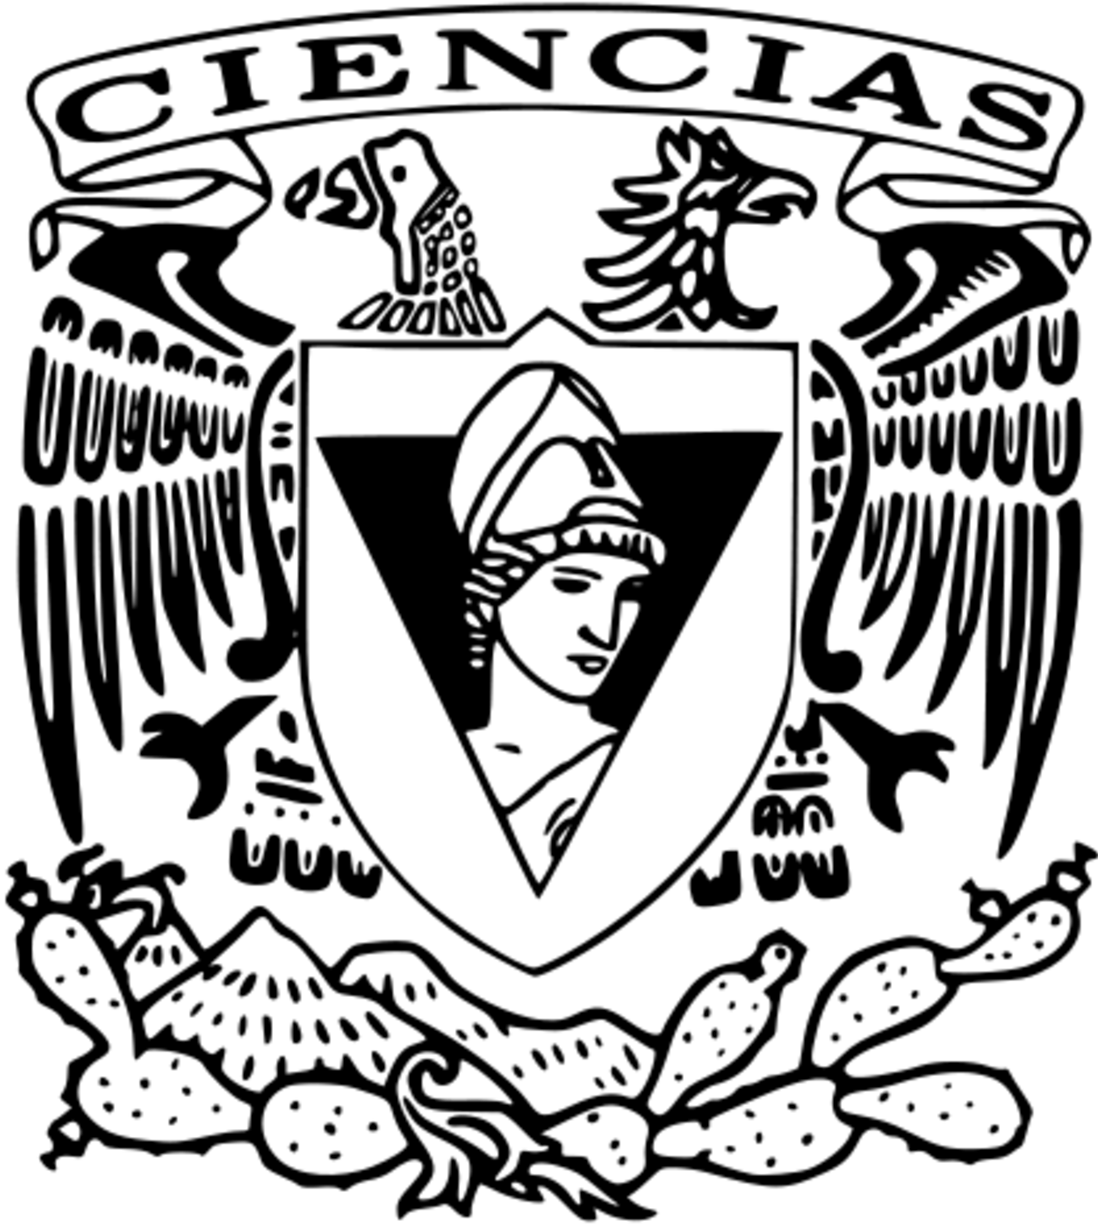
\includegraphics[height=3.4cm]{Logo_FC.png}
            \end{center}
        \end{minipage}
    \end{center}

    \vspace{2cm}
    
    \begin{center}
        {\Huge Práctica 4: Cifrados Clásicos}
    \end{center}
    
    \vspace{2cm}
    
    \begin{center}
        \large

        \textsc{Equipo: \\
                \textbf{Barrientos Sánchez José Antonio\\
                Hernandez Gonzalez Yun\\
                Ortiz Castañeda José Ramón}}\\[0.5cm]     
                
                \textsc{{Fecha de entrega: \\ \textbf{10 de septiembre de 2024}}}\\[0.5cm]        

                \textsc{{Profesor: \\ \textbf{ Anayanzi Delia Martínez Hernández}}}\\[0.5cm]  

                \textsc{Ayudantes: \\\textbf{Cecilia del Carmen Villatoro Ramos \\
                José Angel Arévalo Avalos \\
                Ivan Daniel Galindo Perez \\
                David Armando Silva de Paz}}
    \end{center}
    
    \vfill
    
    \begin{center}
        \rule{17cm}{0.1mm}
    \end{center}
    
\end{titlepage}

\restoregeometry % Restaurar los márgenes originales

\tableofcontents

\section{Introducción}




\section{Desarrollo.}


\section{Preguntas.}

\section{Conclusiones}





\printbibliography




\end{document}
